\setlength{\parindent}{0em}
\section{Sphärische Trigonometrie}
\subsection{Das Kugeldreieck}

Werden drei voneinander verschiedene Punkte, die sich nicht auf derselben Grosskreisebene befinden, mit Grosskreisbögen verbunden, so entsteht ein Kugeldreieck ABC.
A, B und C sind die Ecken des Dreiecks und dessen Seiten sind die Grosskreisbögen zwischen den Eckpunkten. 
Da die Länge der Grosskreisbögen wegen der Abhängigkeit vom Kugelradius ungeeignet ist, wird die Grösse einer Seite mit dem zugehörigen Mittelpunktwinkel des Grosskreisbogens angegeben. 
Laut dieser Definition ist die Seite c der Winkel AMB. 
Für ein Kugeldreieck gilt, dass die Summe der drei Seiten kleiner als $2\pi$ aber grösser als 0 ist. 
Man kann bei Kugeldreiecken nicht so einfach unterscheiden, was Innen oder Aussen ist. 
Wenn man drei Eckpunkte miteinander verbindet, ergeben sich immer 16 Kugeldreiecke. 
Jenes Kugeldreieck mit den Seitenlängen $a, b, c < \pi$ und den Winkeln $\alpha, \beta, \gamma < \pi$ nennt man Eulersche Dreiecke.
\begin{figure}[h]
	\begin{center}
		%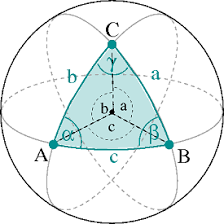
\includegraphics[width=6cm]{papers/nav/bilder/kugel1.png}
		\caption[Das Kugeldreieck]{Das Kugeldreieck}
	\end{center}
	
\end{figure}

\subsection{Rechtwinkliges Dreieck und Rechtseitiges Dreieck}
Wie auch im uns bekannten Dreieck gibt es beim Kugeldreieck auch ein Rechtwinkliges Kugeldreieck, bei dem ein Winkel $\frac{\pi}{2}$ ist. 
Ein Rechtseitiges Dreieck gibt es jedoch nur beim Kugeldreieck, weil dort eine Seitenlänge $\frac{\pi}{2}$ lang sein muss.
\newpage
\subsection{Winkelangabe}
\begin{figure}[h]
	
	\begin{center}
		%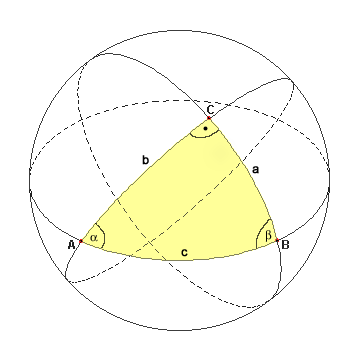
\includegraphics[width=8cm]{papers/nav/bilder/kugel2.png}
		\caption[Winkelangabe im Kugeldreieck]{Winkelangabe im Kugeldreieck}
	\end{center}	
\end{figure}


Die Winkel eines Kugeldreiecks sind die, welche die Halbtangenten in den Eckpunkten einschliessen. 
Für die Summe der Innenwinkel gilt
\begin{align}
	\alpha+\beta+\gamma &= \frac{A}{r^2} + \pi \ \text{und} \ \alpha+\beta+\gamma > \pi. \nonumber
\end{align}

Der sphärische Exzess
\begin{align}
	\epsilon = \alpha+\beta+\gamma - \pi \nonumber
\end{align}  
beschreibt die Abweichung der Innenwinkelsumme von $\pi$ und ist proportional zum Flächeninhalt des Kugeldreiecks.

\subsection{Sphärischer Sinussatz}
In jedem Dreieck ist das Verhältnis des Sinus einer Seite zum Sinus des Gegenwinkels konstant. 

Das bedeutet, dass

\begin{align}
	\frac{\sin (a)}{\sin (\alpha)} =\frac{\sin (b)}{\sin (\beta)} = \frac{\sin (c)}{\sin (\gamma)} \nonumber \ \text{auch beim Kugeldreieck gilt.}
\end{align}



\subsection{Sphärischer Satz des Pythagoras für das rechtwinklige Kugeldreieck}
Es gibt in der sphärischen Trigonometrie eigentlich garkeinen "Satz des Pythagoras", wie man ihn aus der zweidimensionalen Geometrie kennt.
In der sphärischen Trigonometrie gibt es aber auch einen Satz, der alle drei Seiten eines rechtwinkligen Kugeldreiecks in eine Beziehung bringt. 

Es gilt nämlich:
\begin{align}
	\cos c = \cos a \cdot \cos b \ \text{wenn} \nonumber &
	\alpha = \frac{\pi}{2} \lor \beta =\frac{\pi}{2} \lor \gamma = \frac{\pi}{2}.\nonumber
\end{align}
 